\documentclass[12pt]{article}

\usepackage[dvips,letterpaper,margin=0.75in,bottom=0.5in]{geometry}
\usepackage{cite}
\usepackage{slashed}
\usepackage{graphicx}
\usepackage{amsmath}
\usepackage{amssymb}
\usepackage{braket}
\usepackage{accents}
\usepackage{tikz}
\newcommand*{\dt}[1]{%
  \accentset{\mbox{\large\bfseries .}}{#1}}

\begin{document}


\title{PHY 130A \\ Lecture Notes: \\ 
Fermi's Golden Rule }
\author{Michael Mulhearn}

\maketitle

\section{The Interaction Picture}

We consider a time-dependent Hamiltonian of the form:
$$H = H^{(0)} + \delta H(t)$$
where $H^{(0)}$ is time independent and so well understood, with energy eigenstates:
$$H^{(0)} \ket{n} = E_n \ket{n}$$
and the $\delta H(t)$ represents a new interaction.  The new
interaction is time dependent and therefore has no energy eigenstates.

The interaction picture factors out the simple and well-understood
time dependence from $H^{(0)}$ from the to-be-determined time
dependence of $\delta H(t)$ as:
$$\ket{ \Psi(t) } = \sum_m c_m(t) \exp\left( -i \frac{E_m t}{\hbar} \right) \ket{m}$$
The $\{\ket{m}\}$ are still a basis for the full Hamiltonian $H$, even
though they are not eigenstates, so this is certainly a valid
expansion, due to the time dependent coefficients $c_m(t)$.  This
just says that $\ket{\Psi(t)}$ can be expressed at any time as
a sum of basis vectors, which is certainly true.  We will know it is
useful if it simplifies the problem.  Specifically, if the time
dependence in the coefficients is due exclusively to $\delta H(t)$.

Applying the SE:
\begin{eqnarray*}
  i \hbar \frac{\partial}{\partial t} \, \ket{\psi(t)} \; &=& \; H \, \ket{\psi(t)} \\[5pt]
  &=& H^{(0)} \, \ket{\psi(t)} + \delta H(t) \, \ket{\psi(t)} \\[5pt]
\left( i \hbar \frac{\partial}{\partial t} -  H^{(0)}\right) \ket{\psi(t)} \; &=& \; \delta H(t) \ket{\psi(t)} \\[5pt]
\end{eqnarray*}
where we have arranged things in the hope of getting some cancellation on the left hand side:
\begin{eqnarray*}
\left( i \hbar \frac{\partial}{\partial t} -  H^{(0)}\right) \ket{\psi(t)} \; &=& \;
\sum_m \left\{ i \hbar \dt{c_m}(t) + E_m c_m(t) - E_m c_m(t) \right\} \exp\left( -i \frac{E_m t}{\hbar} \right) \ket{m} \\
  &=&
\sum_m \, i\hbar \dt{c_m}(t)  \, \exp\left( -i \frac{E_m t}{\hbar} \right) \ket{m}
\end{eqnarray*}
and indeed we do.  Meanwhile the RHS is:
$$\delta H(t) \ket{\psi(t)} = \sum_m \, c_m(t)  \, \exp\left( -i \frac{E_m t}{\hbar} \right)
\left(\delta H(t) \ket{m}\right)$$
and so we cannot match coefficients term by term in the expansion because:
$$\ket{m} \; \neq \; \delta H(t) \, \ket{m} $$
So changing dummy variables to prepare for what follows:
$$\delta H(t) \ket{\psi(t)} = \sum_n \, c_n(t)  \, \exp\left( -i \frac{E_n t}{\hbar} \right)
\left(\delta H(t) \ket{n}\right)$$
And inserting a complete set:
\begin{eqnarray*}
\left( \delta H(t) \, \ket{n} \right) &=& \left( \sum_m \ket{m}\bra{m} \right) \left( \delta H(t) \ket{n} \right) \\
&=& \sum_m  \braket{m | \delta H(t) | n} \ket{m}
\end{eqnarray*}
And now putting back LHS equal to RHS
$$
\sum_m \, i \hbar \dt{c_m}(t)  \, \exp\left( -i \frac{E_m t}{\hbar} \right) \ket{m}
= \sum_m \sum_n \, c_n(t)  \, \exp\left( -i \frac{E_n t}{\hbar} \right)
\braket{m | \delta H(t) | n} 
$$
Where we can now match term by term to obtain:
\begin{equation}
\label{eqn:cmdot}
\dt{c_m}(t)  = - \frac{i}{\hbar} \sum_n \, c_n(t)  \, \exp\left( i \frac{(E_m - E_n) t}{\hbar} \right)
\braket{m | \delta H(t) | n}  
\end{equation}
This is everything we hoped for!  Notice that $H^{(0)}$ operator does
not appear explicitly in Equation~\ref{eqn:cmdot}.  The unperturbed
Hamiltonian determines the eigenstates $\ket{m}$ and the energies
$E_m$, but its impact on the time-dependence of the coefficients
$c_m(t)$ is solely through the phase factor:
$$\exp\left( i \frac{(E_m - E_n) t}{\hbar} \right)$$
The interaction picture
\footnote{Formally, in the interaction picture the operators evolve as
$$O(t) = {\rm exp}(iH^{(0)}t/\hbar) \; O \; {\rm exp}(-iH^{(0)}t/\hbar)$$
while the states carry the remaining time dependence.  Our derivation
here achieves exactly the same separation of time dependence without
invoking time evolution of the operators.}  has factored out the time
  dependence from the unperturbed Hamiltonian.

\section{First-Order Time-Dependent Perturbation Theory}

\begin{figure}[thb]
\begin{center}
  \begin{tikzpicture}[scale=1]
    \draw[-] (0.0,0.0) -- ++(4.0,0.0) -- ++(0.0,1.0) -- ++(4.0,0.0) -- ++(0.0,-1.0) -- ++(4.0,0.0);
    \node at (4.0,-0.25) {0};
    \node at (8.0,-0.25) {$T$};
    \node at (12.5, 0.0) {$t$};
    \node at (3.8, 1.0) {$V$};
    \node at (-0.5, 0.5) {$\delta H(t)$};
    \node at (2,  -0.75) {$H = H^{(0)}$};
    \node at (6,  -0.75)  {$H = H^{(0)} + V$};
    \node at (10, -0.75) {$H = H^{(0)}$};    
\end{tikzpicture}
\end{center}
\caption{\label{fig:simple-perturbation} The interaction potential $V$
  is time-independent, however, it turns on at $t=0$ and then off at
  $t=T$, making the total Hamiltonian time-dependent.}
\end{figure}

For our purposes, it suffices to consider the simple time-dependent
interaction $\delta H(t)$ shown in Fig.~\ref{fig:simple-perturbation}.
The interaction potential $V$ has no explicit time dependence, but is
turned on at t=0 and off again at $t=T$, making the total Hamiltonian
time dependent.  We will also assume that the initial state is an
energy eigenstate $\ket{i}$ with
$$H^{(0)} \ket{i} = E_i \ket{i}$$
For $t \leq 0$, the interaction is absent, and $\ket{i}$ is a stationary state of total Hamiltonian,
leading to the familiar time dependence:
$$\ket{\Psi(t)} = \exp\left( -i \frac{E_i t}{\hbar}\right) \;
\ket{i} \hspace{2cm} (t \leq 0)$$
This implies that:
\begin{equation*}
c_m(0) = \delta_{mi}
\end{equation*}
However, starting at $t=0$, the interaction turns on and $\ket{i}$ is
no longer a stationary state.  The probability $p$ of observing the
state $\ket{m}$ is given by:
$$p(t) = |c_m(t)|^2 \hspace{2cm} (0 \leq t \leq T)$$ which we can no
longer assume is zero for $m \neq i$, and is time dependent.  At
$t=T$, the interaction turns off.  The states $\ket{m}$ return to
being stationary states of the total Hamiltonian, but the state is no
longer $\ket{i}$.  We now have a probability
$$P_{fi}(T) = |c_f(T)|^2 \hspace{2cm} (t \geq T)$$ of observing the
system in state $\ket{f}$.  We call this, the transition probability
from state $\ket{i}$ to state $\ket{f}$. Notice that is is constant in
time, but it does depend on how long the interaction is left on ($T$).
The interaction potential shakes things up, mixing up the energy
eigenstates, but once it turns off, things stop moving and stay in
place.

Let's further assume that the interaction potential $V$ is small
compared to the time-independent Hamiltonian $H^{(0)}$.

This scenario lends itself to perturbation
theory, where the new interaction $\delta H(t)$ is referred to as the
perturbation.

In the interaction picture, the well-understood Hamiltonian $H^{(0)}$
is generally large compared to the time-dependent additional
interaction $\delta H(t)$.  Starting from the state with no additional
interaction (the unperturbed state) we calculate the effect of the
perturbation as a series of corrections.  Because our perturbation is
time-dependent, we will need time-dependent perturbation theory.  This
topic is covered in PHY 115B, so we will not go into the topic too
deeply.  Fortunately, we can obtain the first-order results in a
simple, intuitive manner.  In the RHS of Equation~\ref{eqn:cmdot}, we make the
approximation:
$$c_n(t) \sim c_n(0) = \delta_{ni}$$
to obtain a first-order estimate:
\begin{equation}
\label{eqn:cmdot-first-order}
\dt{c_m}(t)  = - \frac{i}{\hbar}  \, \exp\left( i \frac{(E_m - E_i) t}{\hbar} \right)
\braket{m | \delta H(t) | i}   
\end{equation}
For any final state $\ket{f}$, we can estimate the corresponding coefficient for $t \geq T$ by an integral:
$$c_f(T) = - \frac{i}{\hbar}  \; V_{fi} \; \int_0^T \exp\left( i \omega_{fi} t \right) \, dt$$
where we define the interaction potential matrix element:
\begin{equation}
V_{mn} = \braket{m|V|n}
\end{equation}
and the angular frequency:
\begin{equation}
\omega_{mn} = \frac{E_m - E_n}{\hbar}
\end{equation}
There is one subtlety, however.  This prescription is only valid for $f
\neq i$.  At first order
$$c_i(t) = 1.$$
Although probability must flow out of the initial state as other
coefficients become nonzero, probabilities are quadratic in the
amplitudes, and $c_i(t)$ only changes at second order.

\begin{figure}[thb]
\begin{center}
{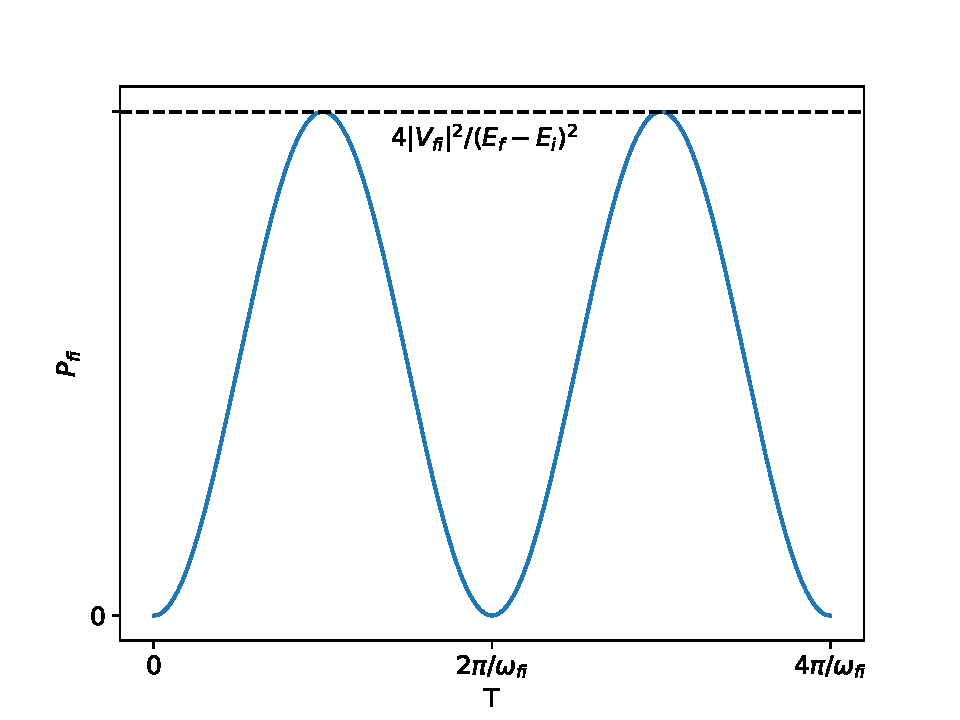
\includegraphics[width=0.60\textwidth]{figs/pfi_osc.pdf}}
\end{center}
\caption{\label{fig:pfi-osc} For $E_f \neq E_i$, the probability $P_{fi}$ oscillates with an amplitude that goes as $1/(E_f-E_i)^2$.}
\end{figure}

Noting that:
$$\int_0^T e^{i\omega t} \, dt = e^{i\omega T/2} \frac{\sin(\omega T/2)}{\omega/2}$$
we determine the first-order transition probability (for $f \neq i$) as:
\begin{equation}
\label{eqn:pfi-first-order}
P_{fi}(T) = |c_f(T)|^2 = \frac{|V_{fi}|^2}{\hbar^2} \; \left( \frac{\sin(\omega_{fi} T / 2)}{\omega_{fi} / 2} \right)^2
\end{equation}
which is plotted in Fig.~\ref{fig:pfi-osc}.  Notice that $T$ appears in the numerator, but not the denominator, of the factor:
\begin{equation}
F_T(\omega_{fi}) = \left( \frac{\sin(\omega_{fi} T / 2)}{\omega_{fi} / 2} \right)^2
\end{equation}
In the next section, we shall see that this factor saves the day for us, twice.  


\section{Fermi's Golden Rule}

In the previous section, we calculated the first-order transition
probability $P_{fi}(T)$, for the probability of a transition from state
$\ket{i}$ to $\ket{f}$, when an interaction was left on for time $T$.
In this section, we will calculate the {\bf rate} at which transitions
occur from the initial state $\ket{i}$ to a collection of final states
in the vicinity of $\ket{f}$ which we shall denote as $\Delta f$.
Conceptually, that rate is:
$$\Gamma_{fi} = \frac{\sum_{\Delta f} P_{fi}(T)}{T}$$
We have no knowledge about the correct value of $T$.
If our result is going to have any utility, $\Gamma_{fi}$ must be
independent of $T$, which can only happen if our first wish is
granted:
\begin{equation}
\sum_{\Delta f} P_{fi}(T) \; \propto \; T
\end{equation}
We shall see if we are so lucky!

For a first step, we'll move to the continuum by the replacement:
$$\sum_{\Delta f} \to \int_{\Delta f} \, dn = \int_{\Delta f} \, \rho(E_f) \, dE_f$$
where the integral is now over a continuous range of final states in
the vicinity of $\ket{f}$, and
\begin{equation}
\rho(E_f) = \left| \frac{dn}{dE_f} \right|
\end{equation}
is the Jacobian of the transformation from $dn$ to $dE$.  More
intuitively, $\rho(E_f)$ is the number of states $dn$ per energy range
$dE$.  We refer to $\rho(E_f)$ as the density of states.  An example
calculation for the non-relativistic case, using box regulation, is in
the Appendix.

Using the main result from the previous section
(Equation~\ref{eqn:pfi-first-order}) we now have:
$$\sum_{\Delta f} P_{fi}(T) = \frac{1}{\hbar^2} \int_{\Delta f} \;
\rho(E_f) \; |V_{fi}|^2 \; \left( \frac{\sin(\omega_{fi} T /
  2)}{\omega_{fi} / 2} \right)^2 \; dE_f$$ At this point, a reasonable
human being would consider giving up.  We don't know anything specific
about the $\rho(E_f)$ and $|V_{fi}|^2$ that appear in the integral,
nor do we know much about the range of integration, which we've
labeled as $\Delta f$, to indicate a continuum in the vicinity of
$\ket{f}$. The only way we can hope to proceed is if there is a delta
function lurking in the integrand, which we shall take as our second
wish.

\begin{figure}[thb]
\begin{center}
{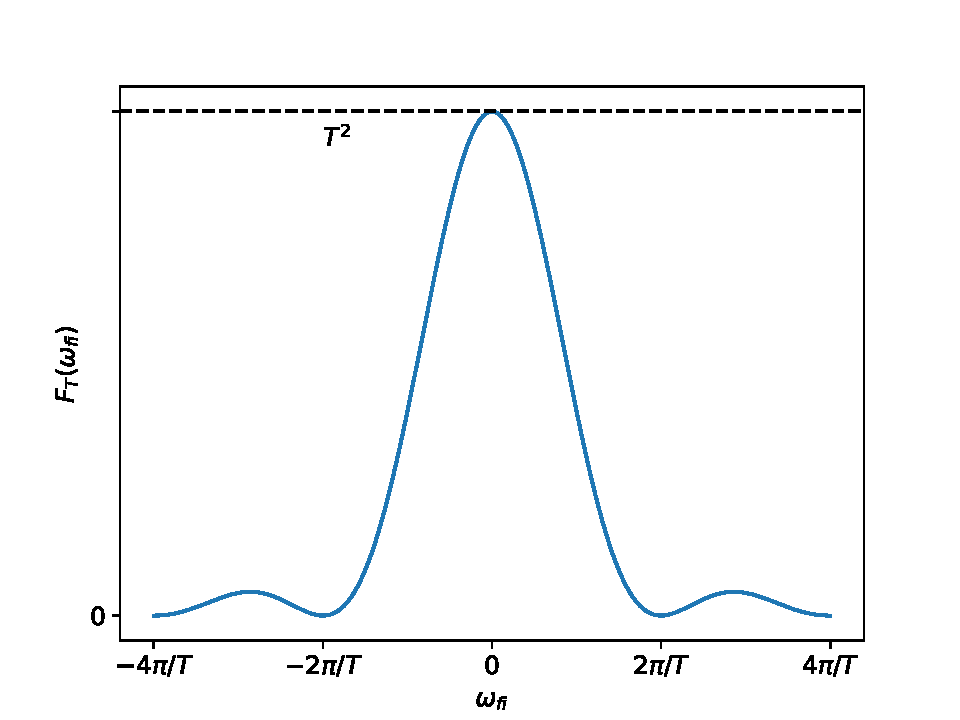
\includegraphics[width=0.60\textwidth]{figs/fgr_delta.pdf}}
\end{center}
\caption{\label{fig:fgr_delta} For large enough $T$, $f(\omega_{fi})$ becomes a delta function and the area under the curve is $\propto T$}
\end{figure}

There is precisely one factor in the integrand which we know
explicitly:
$$F_T(\omega_{fi}) = \left( \frac{\sin(\omega_{fi} T / 2)}{\omega_{fi}
  / 2} \right)^2$$ and it is plotted in Fig.~\ref{fig:fgr_delta}.
Remarkably, it grants both of our wishes.  It has amplitude $T^2$ and
width $\propto 1/T$, so the area is portional to $T$, exactly as we
hoped.  Furthermore, as $T$ increases, the amplitude becomes larger
and the width narrower, so that it approaches a $\delta$-function,
exactly as we hoped.  The delta function sets $\omega_{fi}$ to zero,
which requires $E_f = E_i$.

In light of these developments, we are justified to rewrite our
integral as:
$$\sum_{\Delta f} P_{fi} = \frac{1}{\hbar^2} \rho(E_i) \; |V_{fi}|^2 \;
\int_{-\infty}^{+\infty} \; 
\left( \frac{\sin(\omega_{fi} T / 2)}{\omega_{fi} / 2} \right)^2 \; dE_f$$
where we have taken $E_f = E_i$ and pulled out the constant factors
$\rho(E_f)=\rho(E_i)$ and $|V_{fi}|^2$..  We have also extended the
range of integration of $E_f$ to $(-\infty, +\infty)$, which is
justified because the integral is zero outside of a very narrow range.
The remaining integral is calculable, and yields:
$$\sum_{\Delta f} P_{fi} = \frac{2 \pi}{\hbar} \rho(E_i) \; |V_{fi}|^2 \; T $$
and recalling:
$$\Gamma_{fi} = \frac{\sum_{\Delta f} P_{fi}}{T}$$
we have:
\begin{equation}
\label{eqn:fgr}
\Gamma_{fi} \; = \; \frac{2 \pi}{\hbar} \; \rho(E_i) \; |V_{fi}|^2
\end{equation}
This result is known as Fermi's Golden Rule (FGR), and it is the foundation of
particle physics.

We calculated this result with first-order time-dependent perturbation
theory, so $V_{fi}$ is just the first term in a series that turns out
to be:
\begin{equation}
T_{fi} = \braket{f|V|i} + \sum_{j \neq i} \frac{\braket{f|V|j}\braket{j|V|i}}{E_i-E_j} + \ldots
\end{equation}
Further noting that
$$\rho(E_i) = \left. \left| \frac{dn}{dE_f} \right| \right|_{E_i} = \int \left| \frac{dn}{dE_f} \right| \delta(E_f-E_i) dE_f
= \int \delta(E_f-E_i) dn$$
we can write FGR as:
\begin{equation}
\label{eqn:nrfgr}
\Gamma_{fi} \; = \; \frac{2 \pi}{\hbar} \; \int |T_{fi}|^2 \; \delta(E_f - E_i) \; dn
\end{equation}
The rate of a process is dependent on the transition matrix element squared
($|T_{fi}|^2$) which describes the dynamics of the interaction.  It
also depends on the phase space available, consistent with
conservation of energy: $\delta(E_f - E_i) \; dn$.  In the next
section, will clarify the phase space integral.

\section{Lorentz Invariant Phase Space}

We quantify the phase-space available to a single particle by
integrating over it's available four-momentum:
$$ d^4p \; = \; dp^0 \, dp^1 \, dp^2 \, dp^3 \; = \; dE \, dp_x \, dp_y \, dp_z $$
First, we'll show that this is Lorentz invariant, using our knowledge
of the Lorentz Group.  Recall that the momentum transforms as
$$p^{\mu'} = \Lambda^{\mu'}_\nu p^\nu$$
where the matrix $\Lambda$ with components $\Lambda^{\mu'}_\nu$ is a
member of the Lorentz group.  The Jacobian of a linear
transformation is just the norm of the determinant of the matrix
representing the linear transformation.  So:
$$d^4p' \; = \; |\det \Lambda| \; d^4p$$
Now, the defining property of Lorentz transformations is:
$$\Lambda^T G \Lambda = G$$
where $G$ is the metric tensor.  Using properties of the determinant:
\begin{eqnarray*}
  \det \left( \Lambda^T G \Lambda \right) &=& \det G \\
  \det (\Lambda) \det (G) \det(\Lambda) &=& \det G \\
    \left( \det (\Lambda) \right)^2 \det (G) &=& \det G \\
\end{eqnarray*}
from which it follows that:
$$\det \Lambda = \pm 1$$
Therefore we have:
$$(d^4 p)' = \left| \det \Lambda \right| d^4 p = d^4 p$$
and the four-momentum volume is Lorentz Invariant.

An integral over $d^4p$ will included many different particle masses
via:
$$m^2 = p^\mu p_\mu = (p^0)^2 - (p^1)^2 - (p^2)^2 - (p^3)^2$$
We can restrict our integration to include the particle mass by including a delta function:
$$\delta(p^\mu p_\mu - m^2)$$
since $p^\mu p_\mu$ is Lorentz invariant.  Howerver, this still allows $E = p^0 c$ to run over negative values, so we
also include a $\theta$-function as well:
$$\theta(p^0)$$
Note that $\theta(p^0)$ is not invariant with respect to time
reversal, but it is invariant wrt to rotations (which preserve time)
and boosts (which are linear).  Thus we define the single particle phase-space integral:
$$d\Phi \; \equiv \; \theta(p^0) \; (2 \pi) \, \delta(p^\mu p_\mu - m^2) \; \frac{d^4p}{(2\pi)^4} $$
where we have included factors of $2\pi$ consistent with our
convention for the Fourier transform.  Thus defined $d\Phi$ is
invariant with respect to the {\bf orthochronous} Lorentz Group which
does not include time-reversal (T).  This form of $d\Phi$ makes it's
Lorentz Invariance manifest.  However, there is another way to write
it, more convenient for calculations, by noting:
$$\delta(p^\mu p_\mu - m^2)
= \delta((p^0)^2 - |\vec{p}|^2 - m^2)
= \delta((p^0)^2 - (E)^2)$$
and using this to complete the integral over $dp^0$.  Note the delta function identity (proven below) that:
$$\delta(x^2 - a^2) = \frac{1}{2|a|} \left( \delta(x-a) + \delta(x+a) \right)$$
In this case, we have $p^0 > 0$ so only the first $\delta$ function matters, and we have:
$$d\Phi = \frac{d^3p}{(2E) \; (2\pi)^3}$$
When working with integrals of phase space, we have to be somewhat careful, and recall that $E$ is an integration variable that has been set (via the delta function) to the value
$E = \sqrt{m^2 + |\vec{p}|^2}$ which depends on the other integration values!

In the exercises, you will show that:
\begin{equation}
\label{eqn:invdeltafour}
\delta^4(\Lambda p) = \delta^4(p)
\end{equation}
where $\Lambda$ is a Lorentz transformation.  
That is, the four-dimensional $\delta$-function is Lorentz invariant.\\[4pt]

\noindent
{\bf Exercise:} Verify Equation~\ref{eqn:invdeltafour} using the invariance of $d^4 p$.  Hint: show that:
$$\int \delta (\Lambda p) f(p) d^4 p = \int \delta(p) f(p) d^4 p $$
for an arbitrary function $f(p)$, taking care to note that $p$ is a dummy variable.

\section{Normalization of Momentum Continuum States}

With our single particle Lorentz invariant phase space $d\Phi$
defined, we next want to find a normalization for the momentum
continuum states:
$$\braket{p|p'} \; = \; N(p) \; \delta^3(p-p')$$
consistent with the completeness relation written in Lorentz invariant
form:
\begin{equation}
1 \; = \; \int d\Phi \, \ket{p}\bra{p}
\end{equation}
To do so, we calculate:
\begin{eqnarray*}
\ket{p'} \; &=& \; \int d\Phi \, \ket{p} \braket{p|p'}\\
 &=& \; \int \frac{d^3p}{(2E) (2\pi)^3} \, N(p) \delta(p-p') \, \ket{p} \\
 &=& \; \frac{N(p')}{(2E') (2\pi)^3} \, \ket{p'} \\
\end{eqnarray*}
from which we conclude:
$$N(p) = (2E) \, (2 \pi)^3$$
and  so
\begin{equation}
\braket{p|p'} \; = \; (2E) \, (2 \pi)^3 \; \delta^3(p-p')
\end{equation}

In the exercises, you will show that these results are consistent with
making the substitution:
\begin{equation}
\label{eqn:covsub}
  \ket{p} \to \frac{\ket{p}}{\sqrt{2E}}
\end{equation}
into the corresponding non-relativistic equations.\\[4pt]

\noindent
{\bf Exercise:} Starting from the completeness equation from NR QM:
$$1 = \int \frac{d^3p}{(2\pi)^3} \ket{p} \bra{p},$$
apply the substitution of Equation~\ref{eqn:covsub}, 
read off the phase space integral consistent with the new normalization, and compare to Lorentz Invariant Phase Space.  $\square$\\

\section{Lorentz Covariant Form of Fermi's Golden Rule}

In this section, we'll apply Fermi's Golden Rule to the process
$$a + b + \dots \to 1 + 2 + \ldots$$
so that the initial state is:
$$\ket{i} = \ket{p_a \, p_b \, \ldots} = \ket{p_a} \otimes \ket{p_b} \times \ldots$$
and the final states is:
$$\ket{f} = \ket{p_1 \, p_2 \, \ldots} = \ket{p_1} \otimes \ket{p_2} \times \ldots$$
We'll use a simple notation where
$$\sum E_a = E_a + E_b + \ldots$$
and
$$\sum E_i = E_1 + E_2 + \ldots$$
and similarly for products.  In this context the phase-space integral in Fermi's Golden rule becomes:
\begin{equation}
\label{eqn:nrphin}
(2\pi) \delta(E_f - E_i) dn \to (2 \pi)^4 \delta^4(\sum p_i - \sum p_a) \prod_i \frac{d^3 p_i}{(2\pi)^3}
\end{equation}
where we have included all particles in the final state, but added a
delta function to ensure that three-momentum is conserved.  Note that
no factors of $2 E$ appear, because this is so far a non-relativistic
formulation.

We derived Fermi's Golden Rule by considering a time interval $T$ in
some particular frame.  Fermi's Golden Rule calculates rates.  We do
not expect rates to be invariant under special relativity, and they
are not.  However, we do insist that our results are consistent with
special relativity.  Equations need not be relativistically invariant
in order to be consistent with special relativity.  For example,
four-momentum conservation, e.g.:
$$p_a^\mu + p_b^\mu = p_1^\mu + p_2^\mu$$
is consistent with special relativity because it can be transformed
consistently (e.g. by multiplying both sides by $\Lambda^{\nu'}_\mu$
to obtain:
$$p_a^{\nu'} + p_b^{\nu'} = p_1^{\nu'} + p_2^{\nu'}$$

The values of the four-vectors are frame dependent, but the
relationship between them is not.  The equation
$$p^0 = m$$
is not a covariant equation.  While it might be true in some
particular frame, as $m$ is a scalar and $p^0$ transform as the
temporal part of a four vector, it cannot be true in every frame.

As we derived it, Fermi's Golden Rule is not covariant, but we can
make it so.  Noting that:
$$T_{fi} = \braket{p_a \, p_b \, \ldots | T | p_1 \, p_2 \, \ldots}$$
we can apply the substitution of Equation~\ref{eqn:covsub} to obtain the combined substitution:
\begin{equation}
 \label{eqn:subm}  
 |T_{fi}|^2 \to \frac{|M_{fi}|^2/\hbar^3}{\left( \prod 2\,E_a /\hbar^3 \right) \left( \prod 2\,E_i \right)}
\end{equation}
where $M_{fi}$ is the new Lorentz-invariant matrix element that will replace $T_{fi}$ in our calculations, and the factors of $\hbar$ are worked out in the exercises of Section~\ref{sec:volume-normalization}.  Applying Equations~\ref{eqn:nrphin} and \ref{eqn:subm} to Fermi's Golden Rule as written in Equation~\ref{eqn:nrfgr}, to obtain:
\begin{equation}
\label{eqn:covfgr}
\Gamma_{fi} \; = \; \frac{1}{\hbar^4 \prod (2 E_a/\hbar^3)} \; \int |\mathcal{M}_{fi}|^2 \; (2\pi)^4 \delta^4(\sum p_a - \sum p_1) 
\prod_i \frac{d^3p_i}{(2 E_i) \, (2\pi)^3 }
\end{equation}
The integral is manifestly Lorentz invariant (recall that the four-dimensional $\delta$-function is invariant as in Equation~\ref{eqn:invdeltafour}) so this form of FGR is covariant if $\Gamma_{fi}$ transforms as:
$$\frac{1}{\prod E_a}$$
which, we shall see, is precisely the case.

\section{Two-Body Decays}

We now consider the case of a particle decaying to two particles:
$$a \to 1 + 2$$
in which FGR becomes:
\begin{equation}
\label{eqn:fgr-two-body-decay}
\Gamma_{fi} \; = \; \frac{1}{\hbar 2 E_a} \; \int |\mathcal{M}_{fi}|^2 \; (2\pi)^4 \delta^4(p_1 + p_2 - p_a)
\, \frac{d^3p_1}{(2 E_1) \, (2\pi)^3 } \frac{d^3p_2}{(2 E_2) \, (2\pi)^3 }
\end{equation}
where, as always, we take care that $E_1$ and $E_2$ are functions of
the integration variables.  The integral remains Lorentz invariant, so
the equation is covariant as long as $\Gamma_{fi}$ transforms as
$1/E_a$.  But $\Gamma_{fi}$ is a rate, so transforms as one over the
time-component of a four vector, exactly as $1/E_a$.  Indeed, for this
case at least, we see that FGR is a Lorentz-covariant equation.

Thus convinced of its covariance, we proceed to calculate $\Gamma_fi$ in the rest frame of the particle, where:
$$ E_a = m_a,  \quad \text{and} \quad \vec p_a = 0, $$
so that:
$$\delta^4(p_1 + p_2 - p_a) = \delta(E_1+E_2 - m_a) \, \delta^3(\vec{p}_1+\vec{p}_2).$$
The three-dimensional delta functions kills the integral over $d^3 p_2$, setting:
$$\vec{p}_2 = -\vec{p}_1$$
so that:
$$\Gamma_{fi} \; = \; \frac{1}{32 \pi^2 m_a \hbar} \; \int |\mathcal{M}_{fi}|^2 \; \delta(E_1 + E_2 - m_a)
\, \frac{d^3p_1}{E_1 E_2}$$
Defining:
$$p \equiv |\vec{p}_1|$$
and changing to spherical coordinates:
$$d^3 p_1 = p^2 dp d\Omega$$
we have
$$\Gamma_{fi} \; = \; \frac{1}{32 \pi^2 m_a \hbar} \; \int |\mathcal{M}_{fi}|^2 \; \delta(u - m_a)
\, \frac{p^2 dp d\Omega}{E_1 E_2}$$
where $d\Omega = d\phi d\cos\theta$ is the solid angle and:
$$u \equiv E_1 + E_2$$
Noting that:
$$\frac{du}{dp} = \frac{E_1 + E_2}{E_1 E_2} \, p = \frac{up}{E_1 E_2}$$
and so:
$$\frac{du}{u} = \frac{p\, dp}{E_1 E_2}$$
We now have:
$$\Gamma_{fi} \; = \; \frac{1}{32 \pi^2 m_a \hbar} \; \int |\mathcal{M}_{fi}|^2 \; \delta(u - m_a) \, \frac{p}{u}\, du d\Omega$$
The last delta function kills the integral over u setting:
$$u = E_1 + E_2 = m_a$$
and so:
$$
\Gamma_{fi} \; = \; \frac{p^*}{32 \pi^2 m_a^2 \hbar} \; \int |\mathcal{M}_{fi}|^2  d\Omega$$
where:
$$p^* = |\vec{p}_1|$$
calculated for
$$E_1 + E_2 = m_a \quad \text{and} \quad \vec{p}_2 = -\vec{p}_1.$$
Notice that the $\delta$-functions simply impose four-momentum
conservation.  It is left as an exercise to show that:
\begin{equation}
\label{eqn:pstar}
p^* = \frac{\sqrt{m_a^4 + m_1^4 + m_2^4- 2 (m_a^2 m_1^2 + m_1^2 m_2^2 + m_2^2 m_a^2)}}{2 m_a}
\end{equation}

\noindent
{\bf Exercise:} Verify Equation~\ref{eqn:pstar}.

The decay rate $\Gamma_{fi}$ that we have calculated is independent of
time, as it must be, to be logically consistent with indentical
indistinguishable particles, which cannot, therefore, have any
``age''.  As a result, we have:
$$\frac{dN}{dt} = - \Gamma N$$
with solution:
$$N(t) = N(0) \exp(-\Gamma t) = N(0) \exp(-t /\tau)  $$
where
$$\tau = \frac{1}{\Gamma}$$
is the lifetime of the particle.  The particle lifetime is easily
observable in experiments, for example, by looking at the distance
particles with a known energy travel inside a particle detector before
decaying (accounting for time dilation).

When a particle has multiple decay modes, the total rate is the sum of
all of them:
$$\Gamma_{\rm tot} = \sum \Gamma_i $$
and the particle lifetime is:
$$\tau = \frac{1}{\Gamma_{\rm tot}}$$
Experiments can also measure the branching fraction of a particular
decay: the ratio of the number of observed decays to a particular channel to the total number of decays:
$$Br(a \to x+y) = \frac{N(a \to x+y)}{N(a \to {\rm anything})} = \frac{\Gamma(a \to x+y)}{\Gamma_{\rm tot}}$$

\section{Volume Normalization}
\label{sec:volume-normalization}

Before proceeding, we will need to face an uncomfortable reality.  If
we are going to consider interacting particles, we'll need to consider
the volume that our particles occupy, because the rate at which they
interact will clearly depend on this.  But volume is not Lorentz
invariant.  It turns out, one can just set the volume $V=1$ and
everything works out just fine, and that's the approach that Thomson
takes.  Griffiths evades the topic entirely by just giving FGR for
decays and cross-sections separately without any attempt at a
derivation.  We are going to show how $V$ cancels beautifully when
explicitly accounted for, thus justifying taking Thomson's approach
and simply setting $V=1$ for calculations.

To normalize to one particle per volume $V$ we put:
$$\ket{\Psi} \to \ket{\Psi}/\sqrt{V}$$
Then we need:
$$d\Phi \to V d\Phi$$  
which is no longer Lorentz Invariant.  However:
\begin{equation*}
 \int d\Phi \, \ket{p}\bra{p}
 \to \int V d\Phi \, (\ket{p}/\sqrt{V})(\bra{p}/\sqrt{V})
  \; = \; \int d\Phi \, \ket{p}\bra{p} = 1
\end{equation*}
so when combined with the normalized wave function, the calculations
(at least in this example) are still Lorentz Invariant.

Our calculation of FGR is also modified.  As shown in the Appendix,
the appropriate factor is $V/\hbar^3$, and so:
$$\sum_{\Delta f} \to \int_{\Delta f} \, dn = V \int_{\Delta f} \,
\rho(E_f) \, dE_f$$
So our prescription for modifying the NR FGR becomes:
\begin{equation}
\label{eqn:voltfi}
|T_{fi}|^2 \to \frac{(V/\hbar^3) |M_{fi}|^2}{(\prod 2 (V/\hbar^3) E_a) (\prod 2 (V/\hbar^3) E_i) }  
\end{equation}
and
\begin{equation}
\label{eqn:volps}
(2\pi) \delta(E_f - E_i) dn \to (2 \pi)^4 \delta^4(\sum p_i - \sum p_a) \prod_i \frac{(V/\hbar^3) d^3 p_i}{(2\pi)^3}
\end{equation}
It is left as exercise to show that the volume normalization, when
applied consistently, has no impact on the decay rate calculation.  In
the next section, we will show that for scattering, an additional
volume factor in FGR cancels a volume factor in the flux.\\[4pt]

\noindent
{\bf Exercise:} Set $V=1$ in Equations~\ref{eqn:voltfi} and \ref{eqn:volps}
and apply the substitution to Fermi's Golden Rule as written in Equation~\ref{eqn:nrfgr}.  Show that you obtain Equation~\ref{eqn:covfgr} including the factors of $\hbar$.\\[5pt]

\noindent
{\bf Exercise:} Show that Equation \ref{eqn:fgr-two-body-decay} is unchanged when using the substitutions in Equations~\ref{eqn:voltfi} and \ref{eqn:volps}, which explicitly including the volume factors,instead of Equations~\ref{eqn:nrphin} and \ref{eqn:subm}.\\[5pt]

\section{Interaction Cross-Section}

Next we will consider a scattering process:
$$a + b \to 1 + 2 + 3 + \ldots$$
Eventually, we will arrive at Lorentz Invariant results, but we'll orient ourselves first in a frame where the relative velocities of $a$ and $b$ are collinear, as in:
\begin{center}
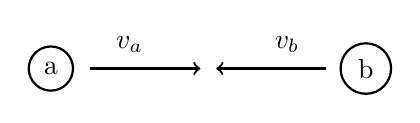
\begin{tikzpicture}[scale=1]
  \node[shape=circle,draw,thick] at (0,0) {a};
  \draw[->, thick] (0.5,0) -- ++(1.4,0);
  \node at (1.0,0.3) {$v_a$};

  \node[shape=circle,draw,thick] at (4,0) {b};
  \draw[->, thick] (3.5,0) -- ++(-1.4,0);
  \node at (3.0,0.3) {$v_b$};
\end{tikzpicture}
\end{center}
Suppose that in a volume $V$, we have $N_a$ particles of type $a$,
each with velocity $v_a$, and $N_b$ particles of type $b$, each with
velocity $v_b$ located in a volume $V$, with velocities all collinear
as in the diagram.  We would expect the rate to scale as:
$$\Gamma \propto (N_a/V)\,(N_b/V)\,V = N_a N_b / V$$ Now suppose
further that the {\it dynamics} of the interaction causing $a$ and $b$
to scatter does not depend on their relative velocity.  The rate of
scattering will scale linear with the relative velocity
$$\Gamma \propto v_a + v_b$$
because $a$ and $b$ particles will encounter one another more frequently.
Putting these effects together we have:
$$\Gamma \propto N_a N_b \frac{(v_a + v_b)}{V} = \frac{(v_a + v_b)}{V}$$
where in the last step we have set $N_a=1$ and $N_b=1$ to consider a single pair of interacting particles.  We define the luminosity
\begin{equation}
\label{eqn:lumi}
L = \frac{v_a + v_b}{V}.
\end{equation}
which contains the factors that influence the rate independently of the dynamics of the interaction.  We define the interaction cross section ($\sigma$) as the proportionality constant between the luminosity ($L$) and the rate ($\Gamma$):
\begin{equation}
\label{eqn:rate-sigma}  
\Gamma = L \, \sigma
\end{equation}
Note that $\sigma$ must have units of area because
$$\Gamma[1/t] = L[1/At] \; \sigma[A]$$
In the exercises, you will show that for elastic scattering of a point
particle on a solid object, the interaction cross-section is quite
literally the cross-sectional area of the solid object.  More
generally, the cross-section is an accounting trick: the rate of a
scattering process is precisely the rate at which particles of type
$a$ and $b$ are brought to within a transverse area $\sigma$ of one
another.

Fermi's Golden Rule determines the rate gamma for the scattering process
$$a + b \to 1 + 2 + 3 + \ldots$$
as:
$$\Gamma_{fi} \; = \; \frac{1}{V} \, \frac{\hbar^2}{ 2 E_a 2 E_b} \;
\int |\mathcal{M}_{fi}|^2 \; (2\pi)^4 \delta^4(\sum p_a - \sum p_1)
\prod_i \frac{d^3p_i}{(2 E_i) \, (2\pi)^3 }$$ where we are (for now)
keeping the volume factors ($V$) explicit, by using the substitutions
in Equations~\ref{eqn:voltfi} and \ref{eqn:volps}.  Unlike the case
for the two-body decay of Equation~\ref{eqn:fgr-two-body-decay}, the
volume factors $V$ do not all cancel at this stage.  The additional
initial state particle brings in one more factor of $V$ which is not
cancelled.  However, using Equations~\ref{eqn:lumi} and \ref{eqn:rate-sigma} we have:
$$\sigma \; = \; \frac{\hbar^2}{4 E_a E_b (v_a + v_b)} \;
\int |\mathcal{M}_{fi}|^2 \; (2\pi)^4 \delta^4(\sum p_a - \sum p_1)
\prod_i \frac{d^3p_i}{(2 E_i) \, (2\pi)^3 }$$
As before, the integral is manifestly Lorentz invariant, so $\sigma$ will transform as $1/F$ where:
$$F = 4 E_a E_b (v_a + v_b)$$
In the exercise below, you will show that $F$ can be written in the
equivalent form (for this particular frame):
\begin{equation}
\label{eqn:lorentz-invariant-flux}
F = 4 \sqrt{(p_a\cdot p_b)^2 - (m_a m_b)^2}  
\end{equation}
which is manifestly Lorentz invariant.\\[4pt]

\noindent
{\bf Exercise:} Calculate the Lorentz invariant phase-space:
$$ F = 4 \sqrt{(p_a\cdot p_b)^2 - (m_a m_b)^2}$$
in a frame where the velocities of $a$ and $b$ are collinear, and show that:
$$F = 4 E_a E_b (v_a + v_b) = 4(E_a p_b + E_b p_a) \quad \square$$

We can therefore write the cross-section as:
$$\sigma \; = \; \frac{\hbar^2}{4 \sqrt{(p_a\cdot p_b)^2 - (m_a m_b)^2}} \;
\int |\mathcal{M}_{fi}|^2 \; (2\pi)^4 \delta^4(\sum p_a - \sum p_1)
\prod_i \frac{d^3p_i}{(2 E_i) \, (2\pi)^3 }$$
which is manifestly Lorentz Invariant.  This is excellent news, as the
interaction cross-section encodes the dynamics of the interactions
between particles $a$ and $b$, and therefore must be Lorentz invariant
as the laws of physics must be the same in all inertial frames.

The interaction cross-section is bread-and-butter experimental and
theoretical particle physics.  It is an excellent experimental handle,
applicable to the center of a star to the surface of our ocean.  In
the simplist form, we aim particles of type $a$ at particles of type
$b$ and count the number that scatter during the course of our
experiment.\\[5pt]


In the exercise below, you will show that in the CMS, the golden rule for the two-body scattering  cross-section is:
\begin{equation}
\label{eqn:fgr-sigma-two-body}
\sigma = \frac{\hbar^2 p_f^*}{64 \pi^2 s p_i^*} \int |\mathcal{M}_{fi}|^2 d\Omega
\end{equation}
where $s = (p_a + p_b)^2$ is the total energy in the CMS.  Hint: show that the 

\noindent
{\bf Exercise: } Show that in the CMS, the Lorentz invariant flux is
$$F = 4 \, \sqrt{s} \, p_i^*$$

\appendix

\section{Density of Final States}
\label{sec:density}
We cannot count continuum states, so we impose a fiction that a free particle is in fact constrained to a box with sides of length $L$ and so:
$$V = L^3$$
We hope that our final results will not depend on this fictitious
volume $V$.  With this in mind, we consider the normalization of the energy eigenstates of the free particle (plane waves) as:
$$\psi(x) = N e^{i k_x x} \;e^{i k_y y} \;e^{i k_z z} $$
If we choose:
$$N = \sqrt{\frac{1}{V}}$$
then:
$$\int_V |\psi(x)|^2 d^3x = 1 $$
Assuming periodic boundary conditions:
\begin{eqnarray*}
  k_x L &=& 2 \pi n_x  \\
  k_y L &=& 2 \pi n_y  \\
  k_z L &=& 2 \pi n_z  
\end{eqnarray*}
so that
$$dn = dn_x dn_y dn_z = \left( \frac{L}{2\pi} \right)^3 dk_x dk_y dk_z$$
and we have:
\begin{equation}
\label{eqn:dndthreek}
dn = \left( \frac{L}{2\pi} \right)^3 d^3k
\end{equation}
in terms of the momentum $p = \hbar k$, we have:
\begin{equation}
\label{eqn:dndthreep}
dn = \frac{V/\hbar^3}{(2\pi)^3} \; d^3p
\end{equation}
which reproduces the single-particle phase-space factors in
Equation~\ref{eqn:volps}, including the factors of $\hbar$.  Note that
in the convention here, $dn$ is dimensionless, consistent with our
framing of the problem as counting discrete states of a particle
constrained to a finite volume $V$.

It is convenient to express Equation~\ref{eqn:dndthreek} as a differential in energy.  As our box size cannot possibly be Lorentz invariant, we'll use the non-relativistic energy of the free particle (for now):
$$E=\frac{(\hbar k)^2}{2 m}$$
so we have:
\begin{eqnarray*}
dk   &=& \frac{m}{\hbar^2 k} dE \\[4pt]
d^3k &=& k^2 dk d\Omega = \frac{m k }{\hbar^2} d\Omega dE \\[4pt]
dn   &=& \left( \frac{L}{2\pi} \right)^3 \left(\frac{m}{\hbar^2 k}\right) d\Omega \; dE
\end{eqnarray*}
where we have identified the (classical) density of states:
\begin{equation}
 \rho(E) \equiv \left| \frac{dn}{dE} \right| = \left( \frac{L}{2\pi} \right)^3 \left(\frac{m}{\hbar^2 k}\right) d\Omega 
\end{equation}
with:
\begin{equation}
 dn = \rho(E) \, dE 
\end{equation}

\section{Math Tools}

In the previous section, we used some math tools.  First, we need to know how to calculate the Jacobian of a coordinate transformation.  Suppose we are calculated an integral:
$$I = \int f(u,w) \; du \, dw$$
but suppose we have some other coordinates $r$ and $s$ with:
\begin{eqnarray*}
  u &=& u(r,s) \\
  w &=& w(r,s) \\
\end{eqnarray*}
then we can calculate our integral in terms of coordinates $r$ and $s$ via:
$$I = \int f( u(r,s), w(r,s) ) \left| \frac{\partial(u,w)}{\partial(r,s)}\right| \; dr \, ds$$
where
\begin{equation*}
\frac{\partial(u,w)}{\partial(r,s)} =
\begin{vmatrix}
  \frac{\partial u}{\partial r} & \frac{\partial u}{\partial s} \\[5pt]
  \frac{\partial w}{\partial r} & \frac{\partial w}{\partial s} \\[5pt]
\end{vmatrix}
\end{equation*}
is the Jacobian:  the determinant of the matrix of partial derivatives.  We can summarize this as:
$$du\,dw = \left| \frac{\partial(u,w)}{\partial(r,s)} \right| \; dr \, ds $$
The result easily extends to more coordinates, e.g.:
$$du\,dv\,dw = \left| \frac{\partial(u,v,w)}{\partial(r,s,t)} \right| \; dr \, ds \, dt$$
where now the Jacobian will be the determinant of 3x3 matrix.

Second, we needed:
$$\delta(x^2 - a^2) = \frac{1}{2|a|} \left( \delta(x-a) + \delta(x+a) \right)$$
There's a trick for finding identities like this, using the Heaviside step function:
$$\theta(x) = \begin{cases} 1 & x > 0 \\ 0 & x < 0 \end{cases}$$
and noting that
$$\int_{-\infty}^x \delta(y) dy = \theta(x)$$
so we can consider the delta function to be the derivative of the Heaviside step function:
$$\delta(x) = \theta'(x)$$
To find our identity, we work out that:
$$\theta(x^2-a^2) = \theta(x-|a|) + (1 - \theta(x + |a|))$$
Take the derivative of both sides:
\begin{eqnarray*}
  \theta'(x^2-a^2) 2x &=& \theta'(x-|a|) - \theta'(x + |a|)\\
  \theta'(x^2-a^2)    &=& \frac{\theta'(x-|a|)}{2x} - \frac{\theta'(x + |a|)}{2x}\\
\end{eqnarray*}
Now identify $\delta(x)$ with $\theta'(x)$ and simplifying:
\begin{eqnarray*}
  \delta(x^2-a^2)    &=& \frac{\delta(x-|a|)}{2x} - \frac{\delta(x + |a|)}{2x}\\
                     &=& \frac{\delta(x-|a|)}{2|a|} - \frac{\delta(x + |a|)}{-2|a|}\\
                     &=& \frac{\delta(x-|a|)+\delta(x + |a|)}{2|a|}\\
                     &=& \frac{\delta(x-a)+\delta(x + a)}{2|a|}\\
\end{eqnarray*}





\end{document}



